\chapter{Enhancement con Fourier}
\section{Trasformata di Fourier continua}
Una funzione arbitraria può essere riscritta come l'integrale in frequenza di funzioni goniometriche elementari (seni e coseni) opportunamente pesati. Questo permette di passare da un dominio spaziale, quello dei campioni del segnale, al dominio di Fourier.

Scriviamo la trasformata di Fourier (FT) indicata con $F$ per un segnale monodimensionale. Considerando tempo $t$ e frequenze $\omega$ continue, è possibile derivare la trasformata di una funzione $f(t)$ (scriviamo $\mathfrak{F}$ per indicare che vogliamo calcolare la traformata di una funzione):
\begin{equation}
	\mathfrak{F}(f(t)) = F(\omega) = \int_{-\infty}^{\infty}f(t)e^{-i2\pi\omega t} dt
\end{equation}
e la sua inversa:
\begin{equation}
	\mathfrak{F}^{-1}(F(\omega)) = f(t) = \int_{-\infty}^{\infty} F(\omega)e^{i2\pi\omega t} d\omega
\end{equation}
Siccome cambia solo il segno dell'esponenziale possiamo derivare la proprietà di \textbf{simmetria}\label{prop:symmetryFT}: se $F(\omega)$ è la trasformata di $f(t)$ allora $f(-\omega)$ è la trasformata di $F(t)$.
\subsection{Trasformate notevoli}
\subsubsection{Impulso}
L'impulso è un segnale che vale 1 in zero e 0 in ogni altro istante. La sua trasformata sarà:
\begin{equation}
	F(\omega) = \int_{-\infty}^{\infty}\delta(t)e^{-i2\pi\omega t} dt = e^{-i2\pi\omega 0} = 1
\end{equation}
Questo significa che l'impulso contiene tutte le frequenze, inoltre ricordando le proprietà della trasformata (\ref{prop:symmetryFT}) la trasformata di una funzione costante è un impulso.

\subsubsection{Gradino}\label{sec:gradino}
\begin{wrapfigure}[7]{r}{.26\linewidth}
	\vspace{-1cm}
	\centering
	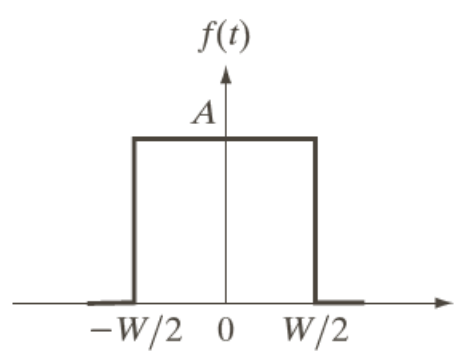
\includegraphics[width=.9\linewidth]{Picture/Step}
	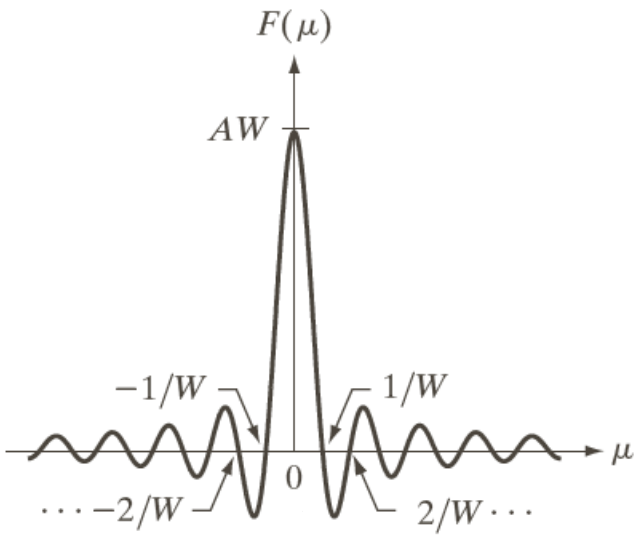
\includegraphics[width=.9\linewidth]{Picture/Sinc}
\end{wrapfigure}
Per una funzione a gradino, definita cioè da:
\begin{equation}
	f(t) = 
	\begin{cases}
		A & if -W/2 \leq t \leq W/2\\
		0 & otherwise
	\end{cases}
\end{equation}
La trasformata è un seno cardinale, cioè
\begin{equation}
	F(\omega) = AW \frac{\sin(\pi\omega W)}{\pi\omega W} = AW\text{sinc}(\omega W)
\end{equation}
\vspace{-.2cm}
\subsubsection{Coseno}
La trasformata del coseno è una coppia di impulsi centrati nell'origine che si trovano uno in $\omega$ (la frequenza del coseno), l'altro in $-\omega$

\subsubsection{Treno di impulsi}
\begin{wrapfigure}[5]{l}{.45\linewidth}
	\vspace{-.7cm}
	\centering
	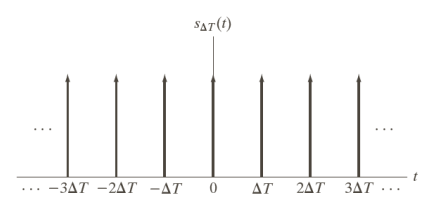
\includegraphics[width=.9\linewidth]{Picture/Impulse_Train}
\end{wrapfigure}
La trasformata di un treno di impulsi è nuovamente un treno di impulsi, se ogni impulso arriva dopo un tempo $\Delta T$, gli impulsi della trasformata si trovano a una distanza di $\frac{1}{\Delta T}$

\subsubsection{Funzioni pari e dispari}
Per le proprietà degli esponenziali una funzione pari trasformata rimane pari e una dispari rimane dispari. Lo stesso vale per l'antitrasformata, che preserva la parità della funzione di partenza.

\subsubsection{Funzioni traslate}
Considero una funzione $f(t)$, la sua trasformata $F(\omega)$ e una traslazione di $t_0$.  Si ottiene
\begin{equation}
	\begin{split}
		\mathfrak{F}(f(t-t_0)) &= \int_{-\infty}^{\infty} f(t - t_0)  e^{-i2\pi\omega t} dt = \\
		&=\int_{-\infty}^{\infty} f(s)  e^{-i2\pi\omega (s + t_0)} ds =\\
		& =e^{-i2\pi\omega t_0} \int_{-\infty}^{\infty} f(s)  e^{-i2\pi\omega s} ds =\\
		&=e^{-i2\pi\omega t_0}F(\omega)
	\end{split}
\end{equation} 
Il risultato è  ottenuto con la sostituzione di variabile $s = t - t_0 \rightarrow t = s + t_0$.

\subsection{Convoluzione}
La convoluzione è una funzione binaria $*$ che si applica a due funzioni $f(t)$ e $h(t)$. La sua definizione è:
\begin{equation}
	f(t)*h(t) = \int_{-\infty}^{\infty} f(\tau) \cdot h(t - \tau) d\tau
\end{equation}
Ricordando il risultato appena ottenuto della trasformata di funzioni traslate possiamo calcolare la trasformata della convoluzione ottenendo:
\begin{equation}
	\mathfrak{F}(f(t) * h(t)) = F(\omega)\cdot H(\omega)
\end{equation}
Cioè la covoluzione diventa un prodotto nel dominio trasformato. Similmente la convoluzione nel dominio di Fourier diventa un prodotto nel dominio del tempo. Questo risultato prende il nome di \textbf{teorema della convoluzione}.

\section{Sampling e DTFT}
Quando acquisiamo digitalmente un segnale, che sia mono o bi dimensionale lo stiamo campionando, è come se lo osservassimo solo in certi momenti. Possiamo quindi vedere il segnale campionato come il segnale originale moltiplicato per un treno di impulsi. La sua trasformata sarà quindi la convoluzione delle trasformate. Chiamiamo questa trasformata DTFT cioè Trasformata di Fourier a tempi discreti e la indichiamo con $\tilde{F}$.
\begin{equation}
	\tilde{F}(\omega) = F(\omega) * S(\omega) = \frac{1}{\Delta T} \sum_{n = -\infty}^{\infty} F(\omega - \frac{n}{\Delta T})
\end{equation}
Dove $S(\omega)$ è la trasformata del treno di impulsi che usiamo per il campionamento (sampling) e, di conseguenza, $\frac{1}{\Delta T}$ è la frequenza di campionamento. Otteniamo cioè infinite copie della trasformata della funzione originale, ciascuna traslata dalla precedente di $\frac{1}{\Delta T}$. 
\subsection{Teorema del campionamento}
Per fare in modo di riuscire a ricostruire fedelmente il segnale di partenza devo fare in modo che le varie copie non si intersechino (sommandosi); significa cioè che la frequenza di campionamento deve essere almeno doppia della frequenza massima presente nel segnale. Questo risultato è noto come \textbf{teorema del campionamento} o di Nyquist-Shannon.

Purtroppo per garantire che le frequenze presenti in un segnale siano limitate questo deve avere durata infinita, dato che questo non può mai verificarsi saremo costretti ad accettare un minimo di sovrapposizione.

\subsection{Aliasing}
Quando le copie della trasformata si sovrappongono si verifica il fenomeno dell'aliasing, ovvero le frequenze più alte del segnale originale vanno ad alterare le frequenze più basse del segnale ricostruito. L'unica soluzione per poter ricostruire il segnale originale è quindi quella di aumentare la frequenza di campionamento.

Quando non è possibile modificare il processo di acquisizione del segnale si possono applicare (prima dell'acquisizione) dei filtri per limitare le frequenze più alte (filtri passa basso).  Questi filtri sono detti anti aliasing, modificheranno il segnale, che non sarà più quello originale, ma spesso questa alterazione è molto minore dell'aliasing. 
\begin{center}
	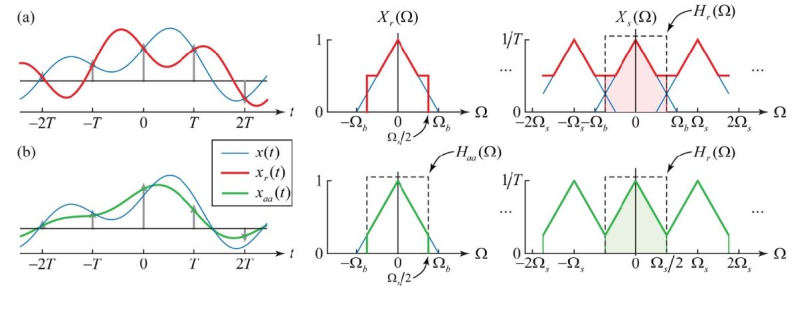
\includegraphics[width=.9\linewidth]{Picture/Aliasing}
\end{center} 
\vspace{-.3cm}
 L'immagine mostra sengale originale (azzurro), ricostruito e trasformata in assenza (a) e presenza (b) di filtri anti alaising, si vede bene come il segnale verde  si avvicini di più all'originale del segnale rosso.
 
 \section{Trasformata di Fourier Discreta}
 Prima abbiamo considerato la trasformata di un segnale a tempi discreti, ora proviamo a discretizzare anche le frequenze e per fare questo consideriamo la periodicità della trasformata $\tilde{F}$ e la campioniamo per un periodo ottenendo M campioni. Si può allora ottenere la Trasformata di Fourier discreta DFT (sia nel dominio dello spazio che della frequenza):
 \begin{equation}
 	F(m) = \sum_{x = 0}^{M-1} f(x)e^{\frac{-i2\pi m x}{M}}
 \end{equation}
 e la sua inversa:
  \begin{equation}
 	f(x) =\frac{1}{M} \sum_{m = 0}^{M-1} F(m)e^{\frac{i2\pi m x}{M}}
 \end{equation}
 Dove sia $x = 0,  1,\dots, M$ che $m = 0,  1,\dots, M$ sono intere e rappresentano rispettivamente gli istanti discreti di tempo e le frequenze discrete.

È facile mostrare che sia la trasformata che l'inversa sono periodiche di periodo $M$. È possibile interpretare la trasformata di Fourier come un cambio di base che ci permette di passare dal dominio spaziale al dominio temporale tramite una matrice di trasformazione (il kernel della trasformata).

\section{Trasformata 2D continua}
Possiamo estendere il concetto di trasformata Fourier al caso bidimensionale ottenendo le seguenti espressioni:
\begin{equation}
	\mathfrak{F}(f(t,z)) = F(u,v) = \int_{-\infty}^{\infty}\int_{-\infty}^{\infty} f(t, z)  e^{-i2\pi (ut + vz)} dt dz
\end{equation}
\begin{equation}
	\mathfrak{F}^{-1}(F(u,v)) = f(t,z) = \int_{-\infty}^{\infty}\int_{-\infty}^{\infty} F(u,v)  e^{i2\pi (ut + vz)} du dv
\end{equation}
Notiamo che siccome le variabili sono indipendenti posso l'integrale è separabile, quindi è possibile integrare prima su una variabile poi sull'altra.

\section{Sampling 2D}
Possiamo ripetere i ragionamenti fatti nel caso monodimensionale quando passiamo al caso bidimensionale. In 2D per campionare non usiamo un treno di impulsi ma una matrice e possiamo ottenere tutti i risultati del caso 1D.
\subsection{Teorema del campionamento}
Possiamo essere sicuri di ricostruire fedelmente un segnale se lo campioniamo a una frequenza almeno doppia della frequenza massima presente nel segnale. Siccome usiamo per acquisire un sensore rettangolare che rappresenta la matrice di impulsi possiamo considerare separatamente frequenze verticali e orizzontali.
\subsection{Aliasing 2D}
Solo funzioni illimitate nel dominio dello spazio sono limitate nel dominio della frequenza, e viceversa, quando acquisiamo un'immagine o un video questo sarà per forza limitato nello spazio e nel tempo, questo porta ad avere un segnale a banda illimitata.

Per quanto detto prima la frequenza di acquisizione sarà sicuramente minore della frequenza massima presente nel segnale. Per limitare il fenomeno dell'aliasing sarà quindi necessario applicare dei filtri passa basso prima dell'acquisizione.
\subsubsection{Aliasing e scalamento}
\begin{wrapfigure}{l}{.63\linewidth}
	\vspace{-.5cm}
	\centering
	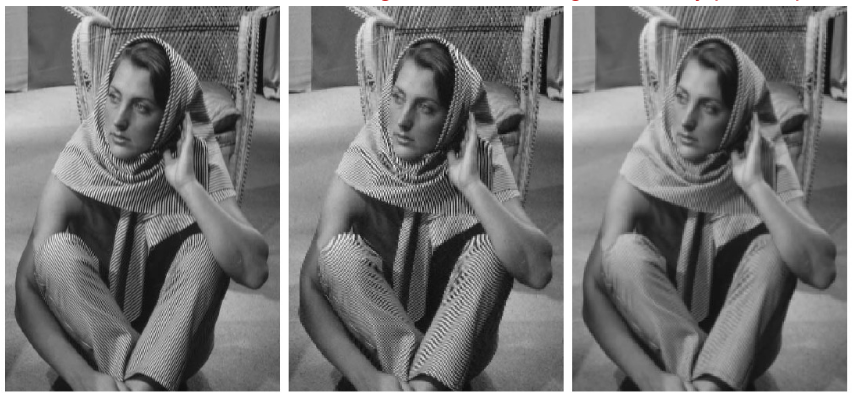
\includegraphics[width=\linewidth]{Picture/Aliasing_Scaling}
\end{wrapfigure}
Quando riduciamo le dimensioni dell'immagine non è sufficiente prendere un pixel ogni due od ogni tre, perché in questo modo si riduce la frequenza di campionamento senza ridurre le frequenze presenti nell'immagine, quindi potrebbero presentarsi artefatti dovuti al rimpicciolimento. Per evitare questo fenomeno è necessario, prima di fare lo scalamento applicare un filtro di blurring che elimini le frequenze troppo alte dall'immagine. Nell'immagine si vede l'immagine originale seguita da un esempio di scalamento prima senza filtro e poi con filtro che elimina le Moirè

\section{Trasformata 2D discreta}
Vediamo ora l'effetto del campionamento sulla trasformata di Fourier:
\begin{equation}
	F(u,v) = \sum_{x=0}^{M-1}\sum_{y=0}^{N-1}f(x,y) e^{-i2\pi (\frac{ux}{M} + \frac{vy}{N})}
\end{equation}
e la sua inversa: 
\begin{equation}
	f(x,y) = \frac{1}{MN}\sum_{u=0}^{M-1}\sum_{v=0}^{N-1}F(u,v) e^{i2\pi (\frac{ux}{M} + \frac{vy}{N})}
\end{equation}
Dove la distanza spaziale tra due campioni orizzontali è $\Delta T$ e tra due campioni verticali è $\Delta Z$, mentre la separazione tra due frequenze orizzontali e verticali è rispettivamente $\Delta u = \frac{1}{M \Delta T}$ e $\Delta v = \frac{1}{N \Delta Z}$

\subsubsection{Modulo e fase}
Come nel caso monodimensionale anche in 2D la trasformata di un \textbf{segnale reale} ha modulo pari e fase dispari.

Se proviamo a fare il plot della fase spesso ci troviamo di fronte un'immagine che pare di puro rumore, nonostante questo è la fase che trasporta le informazioni sulla forma dell'immagine, provando a ricostruire un'immagine solo con la fase si riesce ancora spesso a capire il soggetto, è impossibile invece con il modulo.

\subsection{Traslazioni e rotazioni}
\begin{wrapfigure}{l}{.3\linewidth}
	\vspace{-.5cm}
	\centering
	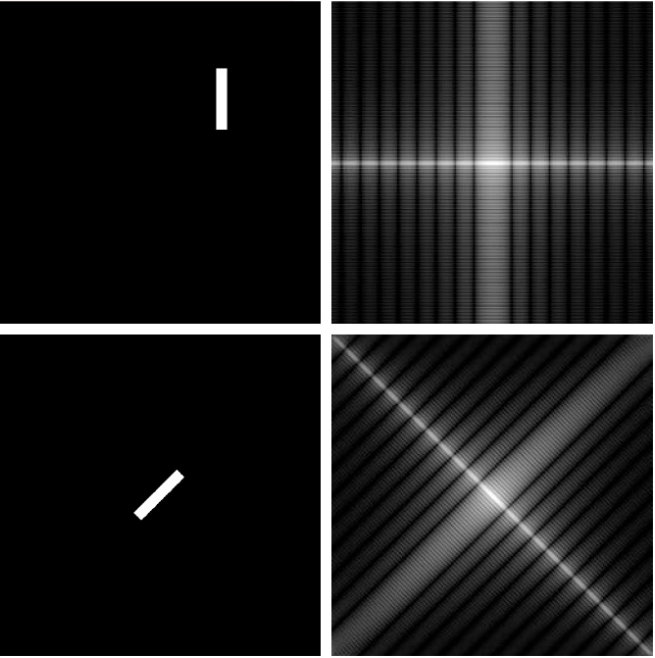
\includegraphics[width=.95\linewidth]{Picture/Rotation_Traslation}
\end{wrapfigure}
La trasformata di Fourier è invariante per traslazione, mentre ruotare l'immagine significa ruotare la trasformata e ruotare la trasformata significa ruotare l'antitrasformata (l'immagine). Nell'esempio si vede prima il rettangolo bianco traslato in alto a destra, che non altera la trasformata, poi il rettangolo ruotato che ha come effetto la rotazione della trasformata.

\subsection{Convoluzione 2D}
In due dimensionei la convoluzione è definita come:
\begin{equation}
	f(x,y) * h(x,y) = \sum_{m=0}^{M-1}\sum_{n=0}^{N-1} f(m,n) h(x-m, y-n)
\end{equation}
Si può dimostrare il \textbf{teorema della convoluzione 2D} che afferma che cambiando dominio la convoluzione diventa un prodotto e viceversa, formalmente si ha che:
\begin{equation}
	f(x,y)*h(x,y)  \Longleftrightarrow F(u,v)H(u,v)
\end{equation}
\begin{equation}
	f(x,y)h(x,y)  \Longleftrightarrow F(u,v)*H(u,v)
\end{equation}

\section{Filtraggio nel dominio della frequenza}
L'idea di base è quella di passare al dominio della frequenza per poter moltiplicare la trasformata del segnale con la trasformata del filtro, poi tornare al dominio spaziale per ottenere il risultato.

\subsection{Zero Padding}
Siccome quando facciamo la trasformata di un segnale 2D di dimensione $N\times M$ otteniamo una trasformata con le stesse dimensioni e per moltiplicare due sengali o due trasformate è necessario che entrambi abbiano le stesse dimensioni dobbiamo fare in modo che i segnali di partenza abbiano la stessa dimensione. Per fare questo possiamo fare \textbf{zero padding}m cioè aggiungere alle funzioni (segnali) degli zeri, in modo che abbiano la stessa dimensione.

Aggiungere degli zeri alla fine di una funzione può però generare componenti di alta frequenza, dato che sarebbe come moltiplicare il segnale per una finestra rettangolare, che abbiamo visto avere un seno cardinale come trasformata (\ref{sec:gradino}); questo fenomeno si chiama \textbf{frequency leakage}.

Per mitigare il frequency leakage al posto che moltiplicare la funzione per un gradino si usano finestre più morbide, che vanno a zero senza salti netti; le finestre più usate sono Gaussiana, di Hann, di Hamming, di Barlett.

\subsection{Progettare un filtro}
Passare al dominio della frequenza ci permette di progettare i filtri in modo nuovo, concentrandoci sulle frequenze e i pattern che vogliamo eliminare dall'immagine.

Purtroppo quando operiamo nel dominio della frequenza dovremmo evitare di creare filtri ideali, dato che questi si traducono in filtri di dimensione infinita nel dominio dello spazio e portano al frequency leakage.

Inoltre quando progettiamo un filtro non vogliamo andare a deformare l'immagine di partenza, dato che l'informazione sulle forme è portata dalla fase della trasformata vorremmo che il filtro non alteri la fase.

In generale quando progettiamo un filtro per un'immagine $f(x,y)$ di dimensioni $M\times N$ dovremmo seguire i seguenti passaggi, che nella maggior parte delle applicazioni portano a dei risultati accettabili:
\begin{enumerate}
	\item fare zero padding dell'immagine arrivando alla dimensione $P\times Q = 2M\times 2N$
	\item moltiplicare l'immagine per $(-1)^{x+y}$ in modo da centrare la trasformata nell'origine
	\item calcolare la trasformata $F(u,v)$
	\item generare il filtro $H(u,v)$ di dimensioni $P\times Q$ centrato in $P/2, Q/2$
	\item calcolare la trasformata del risultato come $G(u,v) = H(u,v)F(u,v)$
	\item calcolare la parte reale dell'antitrasformata e traslarla nell'origine moltiplicando di nuovo per $(-1)^{x+y}$
	\item ritagliare l'immagine alla dimensione $M\times N$
\end{enumerate}